\chapter{Gruppenfilter}\label{gruppenfilter}
\begin{figure}[h!]
	\centering
	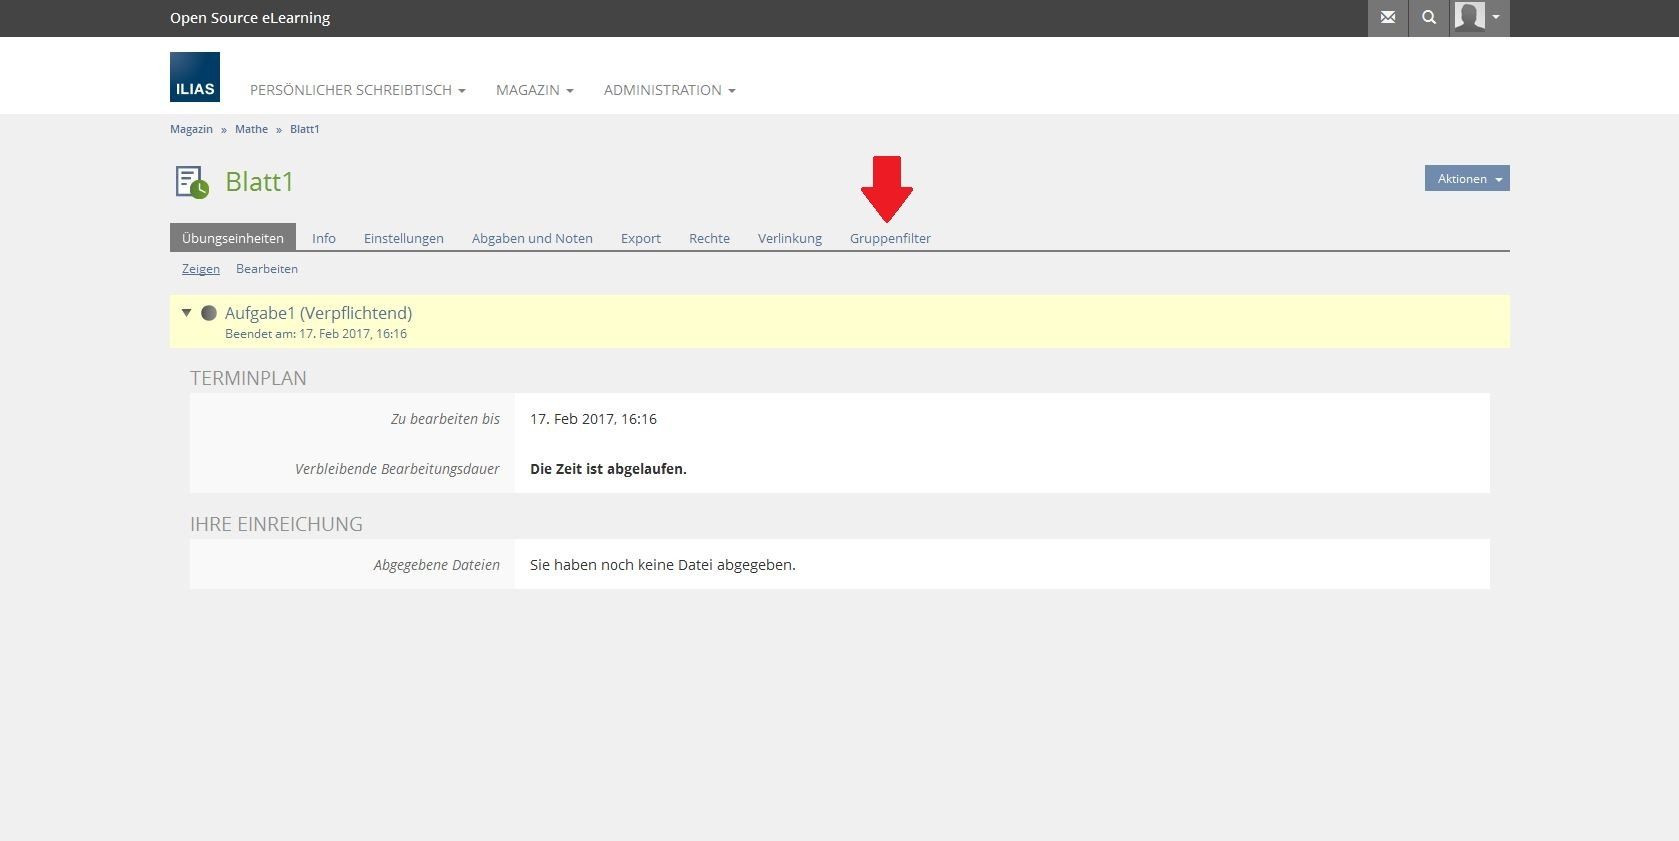
\includegraphics[width=1\textwidth]{img/excerciseGruppenfilter.jpg}
	\caption{Ansicht Gruppenfilter Tab}
\end{figure}

~\\In einer erstellten Übung erscheint für alle Benutzer mit Schreibrechten der neue Tab \textit{Gruppenfilter}. Die Darstellung ist an den ILIAS-Standard Tab \textit{Abgaben und Noten} angelehnt. Allerdings sind etwas weniger Funktionen verfügbar. Das besondere an diesem Tab ist dass man alle Benutzer die Abgaben getätigt haben jetzt nach deren Gruppenzugehörigkeit filtern kann.
\newpage
\section{Gruppenfilter}
\begin{figure}[h!]
	\centering
	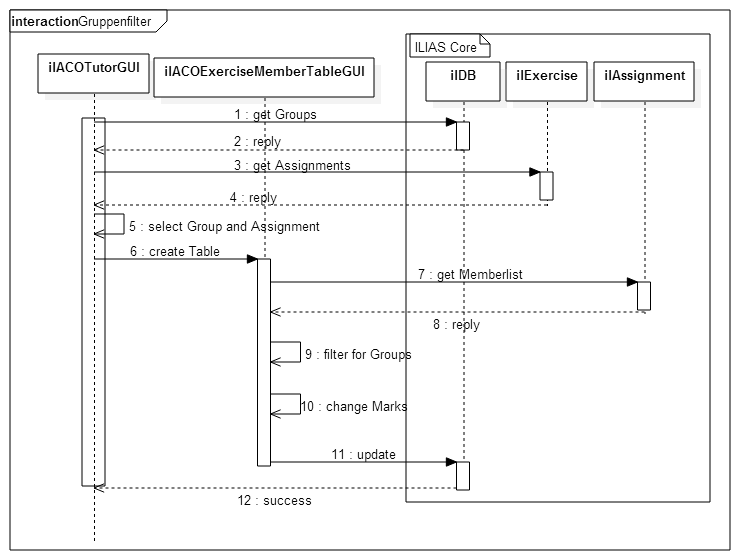
\includegraphics[width=.7\textwidth]{img/seq_tutorGUI.png}
	\caption{Sequenzdiagramm Gruppenfilter}
\end{figure}
\begin{figure}[h!]
	\centering
	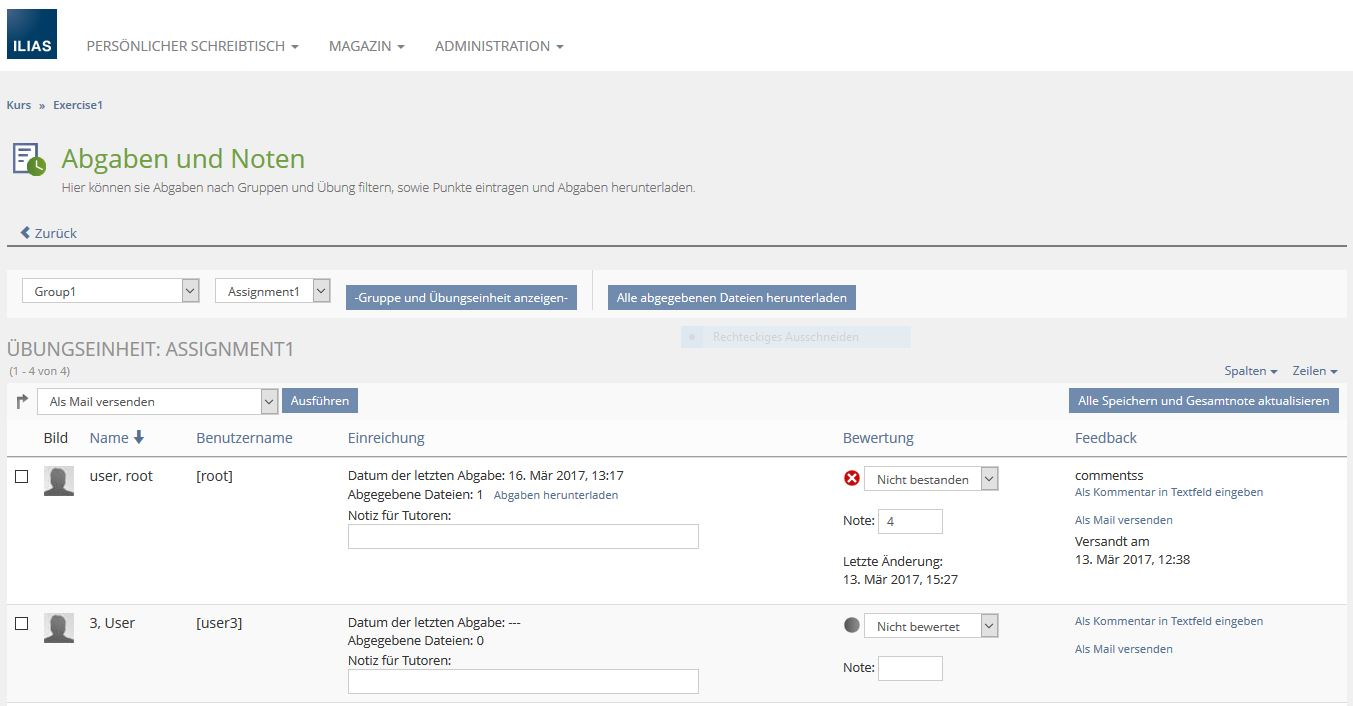
\includegraphics[width=1\textwidth]{img/excerciseGruppentabelle.jpg}
	\caption{Ansicht Gruppenfilter Tabelle}
\end{figure}
~\\Innerhalb von Excercises bzw. Übungen erscheint dieser Reiter/Tab, der es ermöglicht Abgaben nach Gruppen zu filtern. 


\subsection*{Gruppen filtern}
\begin{itemize}
	\item Man wählt in einer Übung den Reiter \textit{Gruppenfilter} aus.
	\item In der Toolbar wählt man jetzt die gewünschte Gruppe und die gewünschte Übungseinheit. Bei nur einer Übungseinheit pro Übung wir kein Auswahlmenü für die Übungseinheit angezeigt. Jeder Benutzer sieht im Auswahlmenü nur die Gruppen in denen er als Administrator festgelegt ist.
	\item Bestätigen mit Klick auf den Button \textit{Gruppe und Übungseinheit anzeigen}
	\item Die Tabelle wird mit den Benutzern der ausgewählten Gruppe gefüllt.
	\item Es bestehen folgende Möglichkeiten der Bearbeitung: 
	\begin{itemize}
		\item Notiz für Tutoren eingeben
		\item Bewertung auswählen
		\item Note eingeben
		\item Feedback als Kommentar eingeben
		
	\end{itemize}
	\item Nach diesen Aktionen bleibt die Tabelle bestehen, bei den Folgenden Operationen wird die Tabelle mit nicht gespeicherten Eingaben verworfen. Es wird daher empfohlen immer zuerst die eingegebenen Daten zu speichern.
	\begin{itemize}
		\item Feedback als Mail versenden
		\item Benutzer zu Teams zusammenfügen (nur bei Abgabetyp Team-Upload)
		\item Teams auflösen (nur bei Abgabetyp Team-Upload)
		\item einzelne Abgabe herunterladen
		\item Alle Speichern und Gesamtnote Aktualisieren
	\end{itemize}
	\item Durch die Bestätigung mit dem Button \textit{Alle Speichern und Gesamtnote Aktualisieren} wird die Gesamtnote der Übung automatisch durch alle enthaltenen Übungseinheiten berechnet.
	\item Danach kann eine weitere Gruppe ausgewählt werden.
\end{itemize}

\clearpage